\chapter{Présentation du projet}

Le jeu de cartes \textit{Dominion} a été mis à disposition sur un serveur de jeu d'octobre 2010 à mars 2013. Les parties effectuées via ce serveur ont été enregistrées dans des \textit{logs} qui mémorisaient toutes les actions des joueurs ; ces \textit{logs} ont été mis à disposition du public. Mais ces enregistrements n'ont pas conservé un certain nombre d'informations ayant un rapport avec les décisions prises par les joueurs.
\newline Un wiki relatif au jeu a été élaboré, et propose des avis d'experts comme aide à la décision pour les joueurs : il propose des conseils, notamment au niveau stratégique. Le but de ce projet, proposé par Yvan Le Borgne, chercheur au Labri, est de traiter ces \textit{logs} (soit plus de 12 millions de parties) afin de répondre à plusieurs interrogations. Il s'agira principalement de comparer Les données recueillies aux préconisations de ce wiki,afin de valider, à travers les contenus des parties, l'éventuelle efficacité des avis et suggestions fournies par les experts. A tout le moins, on cherchera à élaborer des outils de validation présentant une efficacité suffisante.
\newline A cet effet, le projet a pour but de créer une base de données recensant les parties puis un travail d'analyse sera effectuée à partir de celle-ci.
Pour cela notre programme devra tout d'abord extraire les données présentes dans les logs, car ceux-ci sont trop volumineux et trop compliqués à utiliser directement (structure non standardisée). Il s'agira de mettre au point des structures de données permettant de stocker les données de manière plus efficace. Une manière simple de représenter les données extraites et analysées sera proposée à l'utilisateur.
Par ailleurs, il manque des informations dans les enregistrements (\textit{logs}). On cherchera à trouver par quelle méthode on peut les reconstituer et de les mettre dans un format contenant toutes les informations.
En outre, on cherchera à optimiser les opérations menées dans l'analyse des donnnées, en recherchant le meilleur équilibre possible entre la mémorisation des recherches et le re-calcul.
Enfin, on esssaiera de déterminer quelle stratégie a été utilisée dans chaque partie. Voire de faire émerger les changements de stratégie en cours de partie. Si on prend par exemple une des stratégies (la \textit{Penultimate Province Rule}) peut on détecter à quel moment cette règle a été appliquée ou contournée ? ou qui a mis au point cette stratégie ? (découverte qui pourrait permettre d'organiser un classement des joueurs les plus performants) (une sorte de ELO demandé par le client). Dans la mesure où on parviendrait à mettre au point un nombre suffisant de ces démarches stratégiques, il s'agirait de déterminer le processus habituel d'apprentissage des joueurs.

\section{Règles du jeu}
Chaque joueur possède un deck de cartes et a accès à un <<marché>> ou différentes cartes d'action sont disponible. Il y a également une pile de cartes de victoires.
\newline Les joueurs commencent avec un deck contenant uniquement des cartes de monnaie permettant d'acheter les autres cartes mises à la disposition des joueurs. Les joueurs commencent leur tour avec 5 cartes en main et le tour d'un joueur se déroule en deux phases, premièrement la phase d'action, le joueur peut jouer une carte d'action, puis une phase d'achat ou le joueur peut acheter des cartes du marché, des cartes de monnaie ou des cartes de victoires.
\newline La partie se termine dans deux cas, si la réserve de cartes <<Province>> (carte de victoire au score le plus élevé) est vide ou bien si 3 piles du marché sont vides. Quand la partie est terminée, les points de victoires (découlant des cartes de victoire) de chaque deck sont comptés et le vainqueur est celui qui à la meilleur score.


\section{Sujet}

Bla(cf. fig. 1.1)\\

%inclusion d'une mage dans le document
\begin{figure}[!h]
\begin{center}
%taille de l'image en largeur
%remplacer "width" par "height" pour régler la hauteur
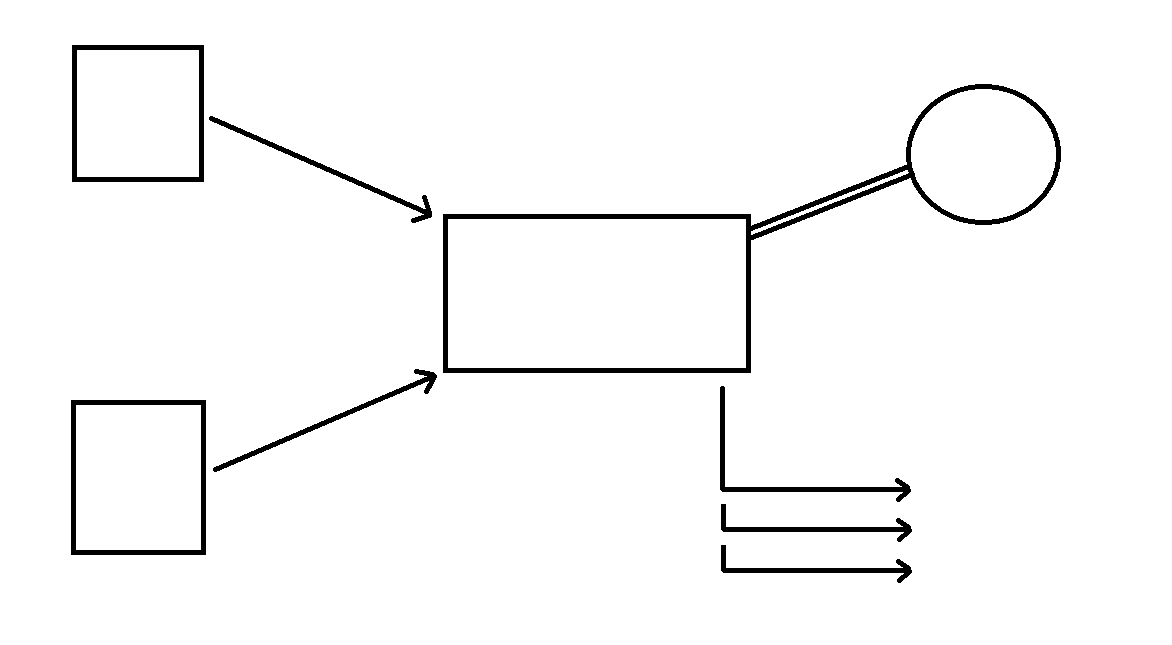
\includegraphics[width=15cm]{presentation/schema}
\end{center}
%légende de l'image
\caption{Schéma descriptif}
\end{figure}

%Contenu de la note précédemment marquée avec \footnotemark
\footnotetext{Note bas de page "intro"}

Bla
%retour à la ligne (alinea)

Bla\\
%saut de paragraphe

Bla

\newpage

\section{Problématique soulevée}

Bla

\begin{center}
Problématique du sujet
\end{center}

\section{Hypothèse de solution}

%Quoi :
Bla\\

Voici une liste :
\begin{itemize}
\item item 1;
\item item 2;
\item item 3;
\item item 4.
\end{itemize}

Bla\\

%Comment :
Bla

Bla\footnotemark\\

%Detail :
Bla(cf. ref. \cite{cite6}).
%citation référencé dans le document "bibliographie.bib" inclus à la fin du document

\footnotetext{Note bas de page "bla"}
